
\tableofcontents

\section{Unit 1: Exploring One-Variable Data}
\subsection{Variation in Categorical and Quantitative Variables}
\subsubsection{Definition}
\begin{definition}
A \textbf{categorical variable} is a variable that can take on one of a limited, and usually fixed, number of possible values.
\end{definition}

\subsubsection{Example Problem}
\begin{example}
Identify whether the following variable is categorical or quantitative: "Type of pet owned."
\end{example}

\subsection{Representing Data Using Tables or Graphs}
\subsubsection{Properties}
\begin{properties}
- Tables can be used to summarize categorical data.
- Graphs such as bar charts and pie charts can visually represent categorical data.
\end{properties}

\subsubsection{Figure}
\begin{figure}[h!]
\centering
\begin{tikzpicture}
\pie[radius=2]{50/A, 30/B, 20/C}
\end{tikzpicture}
\caption{Example of a pie chart.}
\end{figure}

\subsection{Calculating and Interpreting Statistics}
\subsubsection{Theorem}
\begin{theorem}
The mean of a set of data is calculated as the sum of all data points divided by the number of data points.
\end{theorem}

\subsection{Describing and Comparing Distributions of Data}
\subsubsection{Example Problem}
\begin{example}
Compare the distributions of two datasets using histograms.
\end{example}

\subsection{The Normal Distribution}
\subsubsection{Definition}
\begin{definition}
The \textbf{normal distribution} is a continuous probability distribution characterized by a bell-shaped curve.
\end{definition}

\subsubsection{Figure}
\begin{figure}[h!]
\centering
%\includegraphics[width=0.5\textwidth]{normal_distribution.png}
\caption{Normal distribution curve.}
\end{figure}

\section{Unit 2: Exploring Two-Variable Data}
\subsection{Comparing Representations of 2 Categorical Variables}
\subsubsection{Example Problem}
\begin{example}
Create a contingency table to compare two categorical variables.
\end{example}

\subsection{Calculating Statistics for 2 Categorical Variables}
\subsubsection{Properties}
\begin{properties}
- Chi-square tests can be used to determine if there is a significant association between two categorical variables.
\end{properties}

\subsection{Representing Bivariate Quantitative Data Using Scatter Plots}
\subsubsection{Figure}
\begin{figure}[h!]
\centering
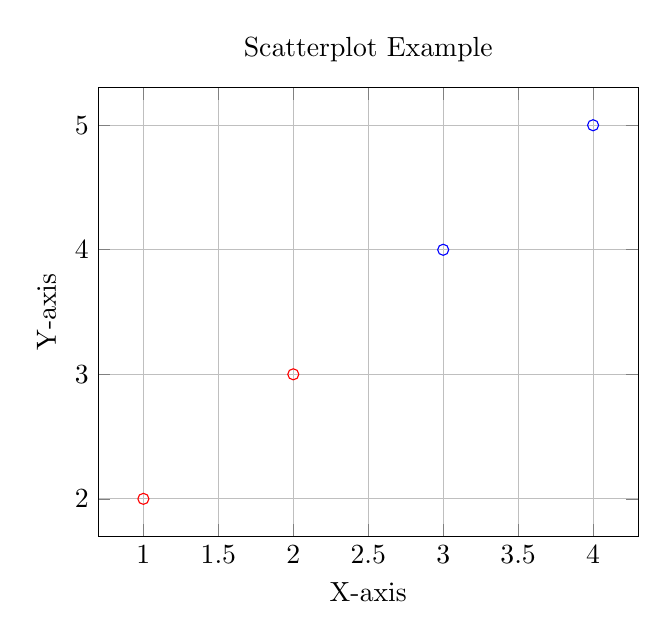
\begin{tikzpicture}
  \begin{axis}[
    title={Scatterplot Example},
    xlabel={X-axis},
    ylabel={Y-axis},
    scatter/classes={
        a={mark=o,draw=red},
        b={mark=o,draw=blue}
    },
    only marks,
    grid=both
  ]
  \addplot[
    scatter,
    only marks,
    scatter src=explicit symbolic
  ]
  table[meta=label] {
      x y label
      1 2 a
      2 3 a
      3 4 b
      4 5 b
  };
  \end{axis}
\end{tikzpicture}
\caption{Example of a scatter plot.}
\end{figure}

\subsection{Describing Associations in Bivariate Data and Interpreting Correlation}
\subsubsection{Theorem}
\begin{theorem}
The correlation coefficient \( r \) measures the strength and direction of a linear relationship between two variables.
\end{theorem}

\subsection{Linear Regression Models}
\subsubsection{Example Problem}
\begin{example}
Fit a linear regression model to a dataset and interpret the slope and intercept.
\end{example}

\subsection{Residuals and Residual Plots}
\subsubsection{Figure}
\begin{figure}[h!]
\centering
%\includegraphics[width=0.5\textwidth]{residual_plot.png}
\caption{Residual plot.}
\end{figure}

\subsection{Departures from Linearity}
\subsubsection{Properties}
\begin{properties}
- Departures from linearity can be identified using residual plots.
\end{properties}

\section{Unit 3: Collecting Data}
\subsection{Planning a Study}
\subsubsection{Definition}
\begin{definition}
A \textbf{study} is a planned investigation designed to answer specific research questions.
\end{definition}

\subsection{Sampling Methods}
\subsubsection{Example Problem}
\begin{example}
Describe the differences between simple random sampling and stratified sampling.
\end{example}

\subsection{Sources of Bias in Sampling Methods}
\subsubsection{Properties}
\begin{properties}
- Bias can occur due to non-random sampling methods.
\end{properties}

\subsection{Designing an Experiment}
\subsubsection{Theorem}
\begin{theorem}
Random assignment of subjects to treatment groups helps to control for confounding variables.
\end{theorem}

\subsection{Interpreting the Results of an Experiment}
\subsubsection{Example Problem}
\begin{example}
Interpret the results of a randomized controlled trial.
\end{example}

\section{Unit 4: Probability, Random Variables, and Probability Distributions}
\subsection{Using Simulation to Estimate Probabilities}
\subsubsection{Example Problem}
\begin{example}
Use a simulation to estimate the probability of rolling a sum of 7 with two dice.
\end{example}

\subsection{Calculating the Probability of a Random Event}
\subsubsection{Theorem}
\begin{theorem}
The probability of an event \( A \) is given by \( P(A) = \frac{\text{Number of favorable outcomes}}{\text{Total number of outcomes}} \).
\end{theorem}

\subsection{Random Variables and Probability Distributions}
\subsubsection{Definition}
\begin{definition}
A \textbf{random variable} is a variable whose possible values are outcomes of a random phenomenon.
\end{definition}

\subsection{The Binomial Distribution}
\subsubsection{Properties}
\begin{properties}
- The binomial distribution describes the number of successes in a fixed number of independent Bernoulli trials.
\end{properties}

\subsection{The Geometric Distribution}
\subsubsection{Example Problem}
\begin{example}
Calculate the probability of the first success occurring on the third trial in a geometric distribution.
\end{example}

\section{Unit 5: Sampling Distributions}
\subsection{Variation in Statistics for Samples Collected from the Same Population}
\subsubsection{Theorem}
\begin{theorem}
The sampling distribution of a statistic is the distribution of the statistic over many random samples from the same population.
\end{theorem}

\subsection{The Central Limit Theorem}
\subsubsection{Definition}
\begin{definition}
The \textbf{Central Limit Theorem} states that the sampling distribution of the sample mean will be approximately normal if the sample size is sufficiently large.
\end{definition}

\subsection{Biased and Unbiased Point Estimates}
\subsubsection{Properties}
\begin{properties}
- An unbiased estimator is one whose expected value is equal to the population parameter being estimated.
\end{properties}

\subsection{Sampling Distributions for Sample Proportions}
\subsubsection{Example Problem}
\begin{example}
Calculate the standard error of the sample proportion.
\end{example}

\subsection{Sampling Distributions for Sample Means}
\subsubsection{Figure}
\begin{figure}[h!]
\centering
%\includegraphics[width=0.5\textwidth]{sampling_distribution.png}
\caption{Sampling distribution of the sample mean.}
\end{figure}

\section{Unit 6: Inference for Categorical Data: Proportions}
\subsection{Constructing and Interpreting a Confidence Interval for a Population Proportion}
\subsubsection{Example Problem}
\begin{example}
Construct a 95% confidence interval for the population proportion based on a sample proportion.
\end{example}

\subsection{Setting Up and Carrying Out a Test for a Population Proportion}
\subsubsection{Theorem}
\begin{theorem}
The test statistic for a population proportion is given by \( z = \frac{\hat{p} - p_0}{\sqrt{\frac{p_0(1-p_0)}{n}}} \).
\end{theorem}

\subsection{Interpreting a p-Value and Justifying a Claim About a Population Proportion}
\subsubsection{Properties}
\begin{properties}
- A small p-value (typically < 0.05) indicates strong evidence against the null hypothesis.
\end{properties}

\subsection{Type I and Type II Errors in Significance Testing}
\subsubsection{Definition}
\begin{definition}
A \textbf{Type I error} occurs when the null hypothesis is rejected when it is actually true.
\end{definition}

\subsection{Confidence Intervals and Tests for the Difference of 2 Proportions}
\subsubsection{Example Problem}
\begin{example}
Construct a confidence interval for the difference between two population proportions.
\end{example}

\section{Unit 7: Inference for Quantitative Data: Means}
\subsection{Constructing and Interpreting a Confidence Interval for a Population Mean}
\subsubsection{Example Problem}
\begin{example}
Construct a 95% confidence interval for the population mean based on a sample mean.
\end{example}

\subsection{Setting Up and Carrying Out a Test for a Population Mean}
\subsubsection{Theorem}
\begin{theorem}
The test statistic for a population mean is given by \( t = \frac{\bar{x} - \mu_0}{s/\sqrt{n}} \).
\end{theorem}

\subsection{Interpreting a p-Value and Justifying a Claim About a Population Mean}
\subsubsection{Properties}
\begin{properties}
- A small p-value (typically < 0.05) indicates strong evidence against the null hypothesis.
\end{properties}

\subsection{Confidence Intervals and Tests for the Difference of 2 Population Means}
\subsubsection{Example Problem}
\begin{example}
Construct a confidence interval for the difference between two population means.
\end{example}

\section{Unit 8: Inference for Categorical Data: Chi-Square}
\subsection{The Chi-Square Test for Goodness of Fit}
\subsubsection{Example Problem}
\begin{example}
Perform a chi-square test for goodness-of-fit to determine if a categorical variable follows a specified distribution.
\end{example}

\subsection{The Chi-Square Test for Homogeneity}
\subsubsection{Theorem}
\begin{theorem}
The chi-square test for homogeneity tests whether the proportions of a categorical variable are the same across different levels of another categorical variable.
\end{theorem}

\subsection{The Chi-Square Test for Independence}
\subsubsection{Properties}
\begin{properties}
- The chi-square test for independence tests whether two categorical variables are independent.
\end{properties}

\subsection{Selecting an Appropriate Inference Procedure for Categorical Data}
\subsubsection{Example Problem}
\begin{example}
Determine the appropriate inference procedure for a given set of categorical data.
\end{example}

\section{Unit 9: Inference for Quantitative Data: Slopes}
\subsection{Confidence Intervals for the Slope of a Regression Model}
\subsubsection{Example Problem}
\begin{example}
\raggedright
Construct a confidence interval for the slope of a regression model.
\end{example}

\subsection{Setting Up and Carrying Out a Test for the Slope of a Regression Model}
\subsubsection{Theorem}
\begin{theorem}
The test statistic for the slope of a regression model is given by \( t = \frac{\hat{\beta}_1 - \beta_1}{SE_{\hat{\beta}_1}} \).
\end{theorem}

\subsection{Selecting an Appropriate Inference Procedure}
\subsubsection{Properties}
\begin{properties}
- The appropriate inference procedure depends on the nature of the data and the research question.
\end{properties}

